\chapter{Container-Runtimes}
\label{chap:compCtnrRuntimes}

Container-Runtimes sind das Herz eines jeden Container-Angebots. Sie instanziieren übergebene Prozesse in isolierten Containern. In diesem Kapitel werden verschiedene Runtimes miteinander verglichen und veranschaulicht, wie Runtimes neben Docker für spezielle Anforderungen besser geeignet sind.

\section{Vorgehen}
\label{sec:vorgehen}
Um verschiedene Runtimes zu vergleichen wurde eine eigene Anwendung mit drei Microservices implementiert. Dabei wurden, wie in \fref{fig:todosStack} zu sehen, verschiedene Technologien verwendet, um zu prüfen, wie die getesteten Container-Runtimes mit diesen umgehen. Diese wurde im Folgenden mit verschiedenen Runtimes bereitgestellt.

\begin{figure}[h]
	\begin{center}
		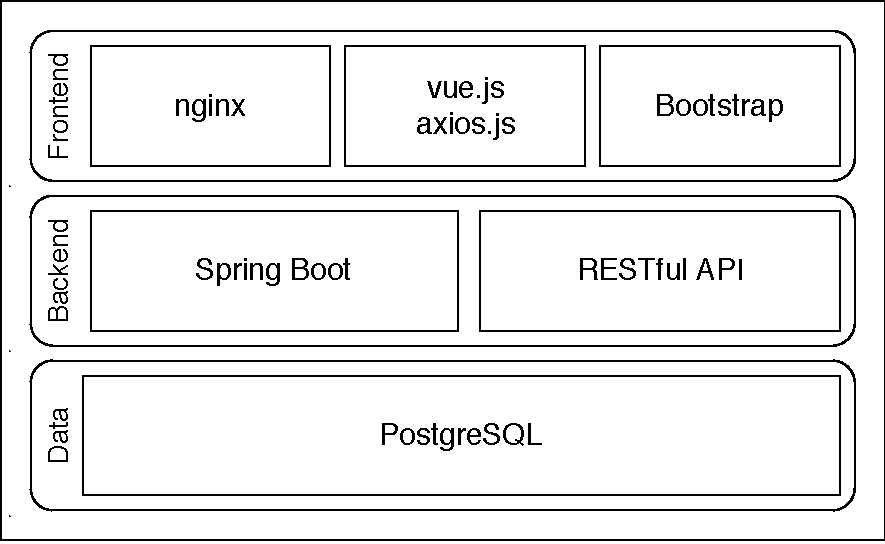
\includegraphics[width=0.7\textwidth]{bilder/microservice-example-stack.pdf}
		\caption{Beispielhafte Darstellung einer Micorservice-Architektur}
		\label{fig:todosStack}
	\end{center}
\end{figure}

\section{Docker Stack}
\label{sec:compDocker}
Docker ist der de facto Standard unter den Container-Technologien und bietet eine vollständige Plattform zur Verwaltung und Orchestrierung von Container (Docker Swarm), der Verbreitung von \glspl{gls-image} (Docker Hub bzw. Docker Store) und der Verwaltung des Container-Lifecycles (Docker CLI) an.

\begin{figure}[h]
	\begin{center}
		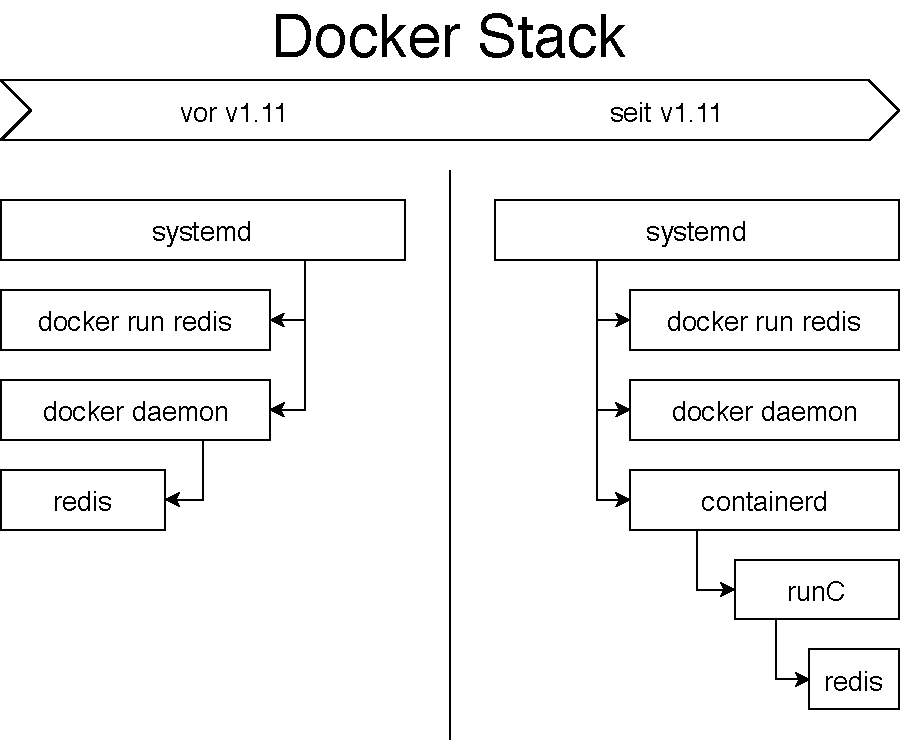
\includegraphics[width=0.9\textwidth]{bilder/docker-stack-containerd-runc.pdf}
		\caption{Docker Stack \citep{RktVsOtherProjects}}
		\label{fig:dockerStack}		
	\end{center}
\end{figure}

Dabei kommen innerhalb des Docker Stacks die Runtimes \texttt{runc} und \texttt{containerd} zum Einsatz. Durch die in \fref{fig:dockerStack} gezeigte Abkapselung der Runtime kann Docker auf jede beliebige \gls{acr-oci}-konforme Runtime aufbauen. Der dadurch gewonnene Vorteil der Kompatibilität bietet allerdings auch Nachteile. Falls einer der vielen Komponenten im Container-Stack einen Bug aufweist, ist das Debugging der Anwendung deutlich komplexer und Fehler können langsamer gefunden werden. Zudem benötigt der Docker-Daemon privilegierte Berechtigungen um die in \fref{sec:funktionsweise} beschriebenen Konzepte zu Nutzen. Da der Daemon auch für den Download und Bau-Prozess der Images zuständig ist, werden alle Images in Docker im Kontext des Users \texttt{root} erstellt.

\subsection{Vorgehensweise}
\label{sec:compDockerVorgehen}

Um den beispielhaften Microservice aus \fref{fig:todosStack} zu Container wurde zuerst für jeden Service ein Image erstellt und diese dann in Containern gestartet. Um dieses Vorgehen zu erleichtern wurde danach \texttt{docker-compose} genutzt, um alle Container in einer Datei zu spezifizieren. Folgend werden beide Wege genauer beschrieben und Vor- bzw. Nachteile dieser Vorgehensweisen aufgezeigt.

Docker verwendet zur Beschreibung eines Images das Dockerfile. Dieses verwendet spezifische Keywords, um Docker beim Bau eines Images zu steuern (\fref{lst:dockerfileExmpl}).

\begin{listing}[h]
	\begin{minted}[xleftmargin=-75pt,breaklines]{dockerfile}
		FROM openjdk:9-jre
		VOLUME /tmp
		ADD ./target/todos-backend-0.0.1-SNAPSHOT.jar app.jar
		EXPOSE 8080
		ENTRYPOINT ["java","-jar","/app.jar"]
	\end{minted}
	\caption{Beispiel für ein Dockerfile}
	\label{lst:dockerfileExmpl}
\end{listing}

Dabei wird deklariert, von welchen Baseimage das neue Image erzeugt werden soll (\textbf{FROM}), welche Änderungen an diesem Image vorgenommen werden müssen (\textbf{VOLUME, ADD, EXPOSE}) und welchen Prozess der Container Isolieren soll (\textbf{ENTRYPOINT}). Dieses Vorgehen erlaubt es einfach, neue Container auf Basis andere zu erzeugen und diese für Dritte zu Verfügung zu stellen. Zu diesem Zweck bietet Docker den Docker Hub an, der als Standardrepository im Docker Stack verwendet wird. Dieser hostet mittlerweile mehr als 100 offizielle Images und eine Vielzahl von Images, die aus der wachsenden Docker Community kommen. Um die in \fref{fig:todosStack} gezeigte Anwendung zu Containern benötigt man somit drei Dockerfiles. Nach dem anlegen der Dockerfiles kann mit dem Befehl \mintinline[breaklines]{bash}{docker build -t <name of image>:<version of image> <path to dockerfile>} das entsprechende Image erstellt werden. Diese Images können mit \mintinline[breaklines]{bash}{docker run <name of image>:<version of image>} containerisiert werden. Durch diesen Prozess kann die gesamte in \fref{fig:todosStack} gezeigte Anwendung in wenigen Minuten gestartet werden.

Vereinfacht wird dieser Prozess mit dem Tool \texttt{docker compose}. Dieses erlaubt es in einer \gls{acr-yml}-Datei alle benötigten Container Images zu spezifizieren und mit dem Befehl \mintinline{bash}{docker-compose up} zu starten (siehe \fref{lst:dockerComposeTodos}).

\begin{listing}[h]
	\begin{minted}[breaklines]{yaml}
version: '3'
services:
 data:
  image: library/postgres
  environment:
   POSTGRES_USER: docker
   POSTGRES_PASSWORD: docker
   POSTGRES_DB: todos
 back:
  build:
   context: ./backend
   ports:
    - "8080:8080"
   environment:
    POSTGRES_PORT: 5432
    POSTGRES_IP: data
 front:
  image: nginx:latest
  ports:
   - "80:80"
  volumes:
   - ./frontend:/usr/share/nginx/html
	\end{minted}
	\caption{docker-compose.yaml für Micorservices}
	\label{lst:dockerComposeTodos}
\end{listing}

Der größte Unterschied liegt dabei in der Art und Weise, wie Container innerhalb des Compose-Clusters angesprochen werden können. Jeder Container bekommt zu seiner IP einen DNS Eintrag mit dem Namen des Service im docker-compose.yml. Dadurch lassen sich die Services einfacher miteinander verknüpfen, da die IP des Containers nicht bekannt sein muss.

\subsection{Bewertung}
\label{sec:compDockerBewertung}
Docker erlaubt es einfach, den Service in Containern bereitzustellen. Dabei ist vor allem das große Vorhandensein bereits bestehender Images verantwortlich, aber auch die einfache Nutzung durch Docker Compose. Das Imageformat für Dockerfiles ist zwar einfach, aber grade für Unixsysteme ungewöhnlich und nur manchmal nur mit Dokumentation nutzbar. Die Vorteile beim einfachen Nutzen kommen allerdings zu einem Preis: Sicherheit. Images auf dem Dockerhub sind nicht verifizierbar und können Schadware und Sicherheitsprobleme mit sich bringen. Die einfache Nutzung des Netzwerks erlaubt ungewollten Zugriff auf containerisierte Services, da jedes Paket an den entsprechenden Container gesendet werden kann. Zudem baut Docker jedes Image unter dem Nutzer root, wodurch potentielle Sicherheitsrisiken wie falsch konfigurierte AppArmor Profile nicht beim Bau-Prozess auffallen.

Notes:
\begin{itemize}
	\item gedacht für Apps
	\item kein extra Tooling
\end{itemize}

\section{rkt}
\label{sec:compRkt}
Notes
\begin{itemize}
	\item unixesque CLI
	\item kein Zentraler Deamon, dadurch integrierbar in init system
	\item gedacht um einzelne Apps zu deployen, nicht ganze Linux Systeme
	\item kaum bis kein wissen über Kernel notwendig
	\item AppC Standard, Docker images, OCI bundles
	\item CNI Networking, CNCF Standard
	\item Secure, crypto validierung default
	\item Jedes Images SOLLTE signiert sein, sichere Quellen
	\item kein root zur laufzeit benötigt
\end{itemize}

\section{LXD / LXC}
\label{sec:compLXD}
Notes:
\begin{itemize}
	\item Gedacht für volle Linux Distros, nicht unbedingt Apps
	\item in Verbindung mit Docker, statt direkte Konkurenz
	\item LXD = LXC + RESTful API
	\item Docker bis anfang 2014 based of LXC
	\item komplexer zu nutzen, da lower Level
	\item Network zwischen Containern nur mit Linux mitteln, wissen von Nöten
	\item Betroffen von Linux-Kernel issues, keine Abstarktion
	\item RESTful API nutzbar über Netz, steuerung ohne SSH, Access zu VM, ...
\end{itemize}

\section{runC}
\label{sec:compRunc}

Notes:
\begin{itemize}
	\item OCI stdimpl
	\item Low Level
	\item OCI bundles, mehrere Dateien zur Steuerung (config json, rootfs tar)
	\item Trend zu std, docker impl
	\item keine Versicherung durch Signatur / Verschlüsselung
	\item CRI-O für Kubernets
\end{itemize}

\section{VM basierte Runtimes}
\label{sec:compVMbased}

Notes:
\begin{itemize}
	\item Mehr sicherheit, seperation Kernel
	\item Weniger Performance, Einzelne Aufrufe, starten und stoppen, ... "teurer" 
	\item Erklären KataContaienrs, gVisor (neue Runtime)
\end{itemize}

\section{Fazit}
\label{sec:compFazit}